\documentclass{ttisummary}

\usepackage{luatexja}
\usepackage{amsmath}
\usepackage{graphicx}
\usepackage{scrextend}
\usepackage{tabularx}

\makeatletter
\let\tti@includegraphics\includegraphics
\renewcommand{\includegraphics}[1]{\tti@includegraphics[width=\linewidth]{#1}}
\makeatother


\title{文書・文間及びカテゴリ間の関係を考慮したレーティング予測}
\author{外山 洋太}



\begin{document}

\section{序論}

企業は、自社商品の市場での評判を常に分析している。
商品の評価レーティング予測は評判分析の重要な要素技術の一つである。
その中でも、商品レビューによるレーティング予測ではレビュー内の言語要素間の
多様で複雑な関係を考慮することが必要である。
特に、複数カテゴリにおけるレーティング予測に関する従来手法\cite{fujitani15}は
文間やカテゴリ間の関係を十分に考慮できていなかった。
本研究は、複数カテゴリにおける評判分類について、
文書及び文間の関係とカテゴリ間の関係を同時に考慮した分類の実現を目的とする。



\section{関連研究}

\subsection{隠れ状態を用いたホテルレビューのレーティング予測}

藤谷ら\cite{fujitani15}は複数のカテゴリにおける評判分類問題に対して、
Multi-Instance Multi-Label learning for Relation Extraction (MIML-RE)
\cite{mihai12}モデルを用いた手法を提案している。
藤谷ら\cite{fujitani15}は、文毎のレーティングからレビュー全体の
レーティングを予測する際のカテゴリ間の繋がりを手調整によって変化させ
カテゴリ間の関係性を考慮している。
しかし、この手法は文同士の位置関係を考慮していない。
また、カテゴリ間については考慮しているものの複雑な関係性を捉えられていない。


\subsection{パラグラフベクトル}

文や文章といった大きな単位の言語表現の分散表現を学習する手法\cite{quoc14}
である。
その手法の一つ、Distributed Memory model of Paragraph Vectors (PV-DM)
によって得られたパラグラフベクトルは評判分類問題において
高い正答率を示している\cite{quoc14}。
しかし、文書全体にパラグラフベクトルを用いる場合、文同士の位置関係が
分類時に考慮できない。


\subsection{ニューラルネットワークを用いた評判分析}

ニューラルネットワークを用いた評判分析の手法が、Nalら\cite{nal14}、
Rieら\cite{rie14}、Duyuら\cite{duyu15}等によって提案されている。
これらの方法に共通するのは、単語の意味表現から畳み込みニューラルネットワークと
全結合ニューラルネットワークを用いて分類を行うことである。

これらの手法は1つのカテゴリにおける分類問題を対象としている。
つまり、多カテゴリの評判分類問題において、これらの手法により
1カテゴリ毎に分類問題を解くだけではカテゴリ間の関係を考慮できない。



\section{提案手法}

\begin{figure}[t!]
  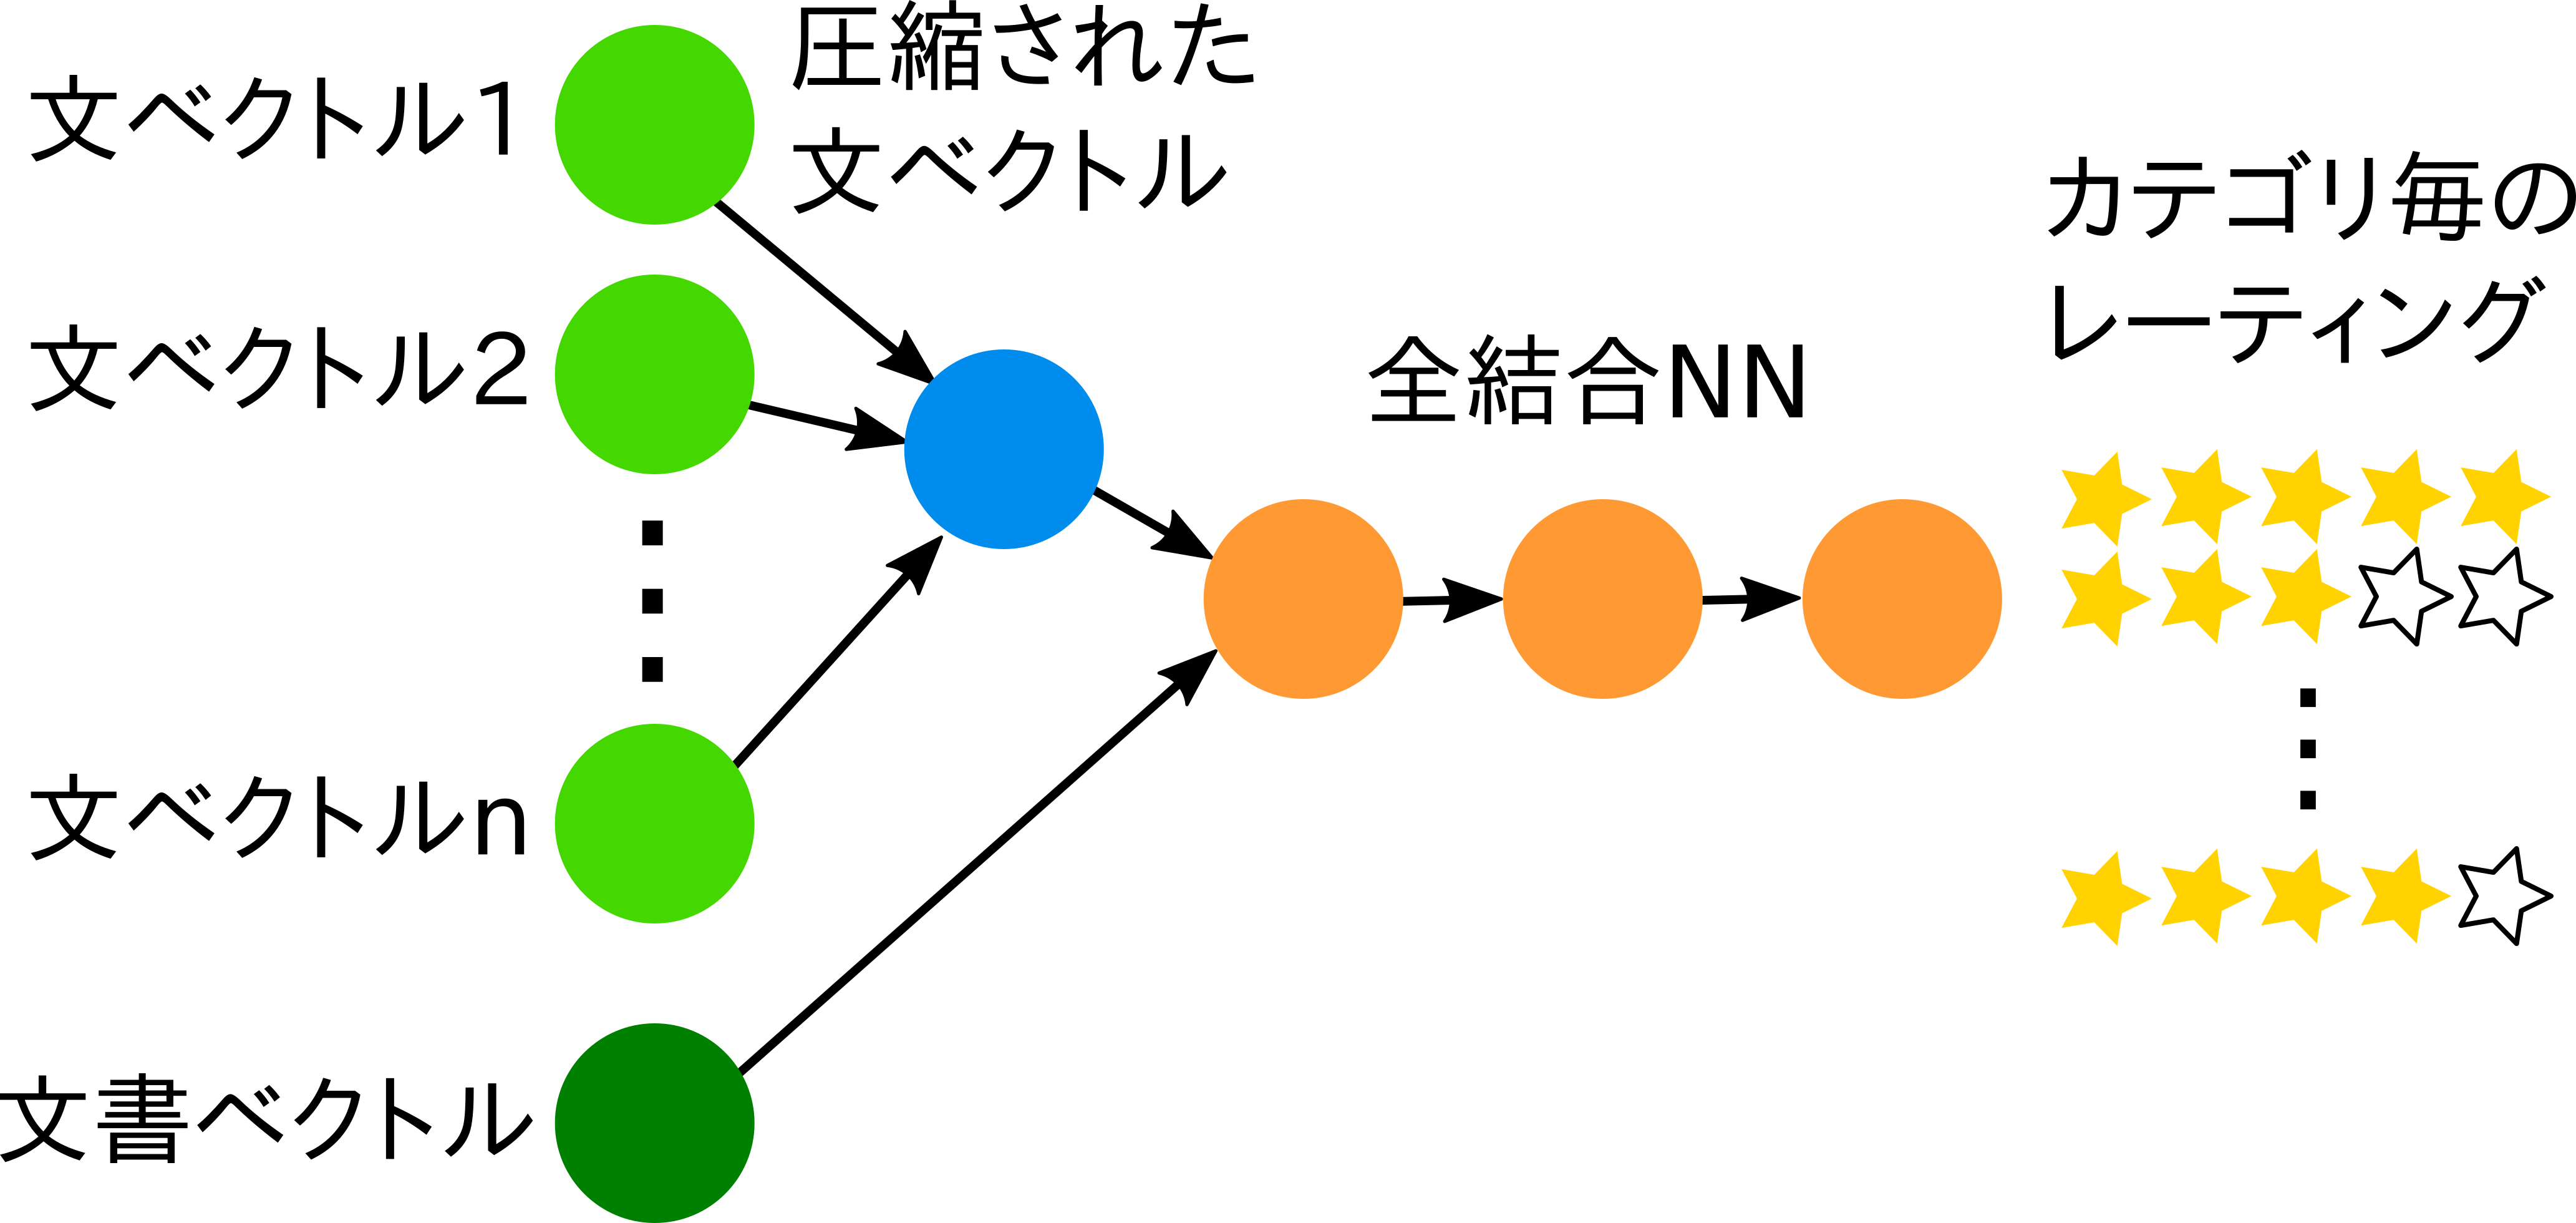
\includegraphics{fig/model.png}
  \caption{提案手法による分類モデルの概略}
  \label{fig:MyModel}
\end{figure}

PV-DMによってレビュー内の文書全体及び各文の分散表現を
生成し、それらをニューラルネットワークの入力として分類を行う手法を提案する。
文毎の意味表現を用いることで文同士の位置関係を考慮し、
全結合ニューラルネットワークによる分類器を用いることで
文間及びカテゴリ間の複雑な関係性を捉えることを目指す。
提案手法の入力はレビューである文書と正解レーティングの組の集合、
出力は各文書について予測されたカテゴリ毎のクラスである。

図\ref{fig:MyModel}にモデルの概略を示す。
提案手法は、まず、PV-DMによって各レビューとそれに含まれる文の意味表現となる
ベクトルを生成する。
次に、各レビュー内の文ベクトルはレビュー毎に重み付け平均によって圧縮する。
この過程により、レビュー毎に疎らだった文の数を統一する。
最後に、レビュー毎の文書ベクトルと圧縮された文ベクトルの
結合ベクトルを分類器の入力層として分類を行う。
出力層の各ニューロンの出力値はあるカテゴリにおけるあるクラスの
正規化されていない対数確率を表す。



\section{実験}

\subsection{実験設定}

実験では、提案手法が従来手法より優れていること、
及び、文書ベクトルと文ベクトルを同時に用いることが
評判分類に有効であることを示すため、各手法の正答率を測定した。
比較手法として、(1) Quocら\cite{quoc14}によるPV-DM、
提案手法における分類器の入力を
(2) ASV (Averaged Sentence Vector)に変えた手法と
(3) Weighted ASVに変えた手法を用いた。
ASVとはレビュー内で平均した文ベクトルであり、
Weighted ASVとはレビュー内で重み付け平均によって圧縮された文ベクトルである。
データセットには、先行研究\cite{fujitani15}と同一の
楽天トラベルにおけるレビューデータを用いた。

\subsection{結果と考察}

\begin{table}[b!]
  \caption{各手法における正答率}
  \centering
  \begin{tabular}{l | r} \label{tab:Accuracies}
    手法 & 正答率 \\
    \hline
    従来手法\cite{fujitani15}  & 0.4832 \\
    PV-DM & 0.4980 \\
    ASV & 0.4838 \\
    Weighted ASV & 0.4867 \\
    提案手法 & \textbf{0.5030} \\
  \end{tabular}
\end{table}

提案手法と3つの比較手法、従来手法\cite{fujitani15}を
正答率で比較したものを表\ref{tab:Accuracies}に示す。
提案手法が従来手法\cite{fujitani15}の正答率を
0.0198上回っていることから、提案手法が従来手法\cite{fujitani15}より
正答率において優れていることが分かった。
また、Weighted ASVの正答率がASVの正答率を0.0029上回っていることから、
文の位置関係の考慮がレーティング予測に有効であることが分かった。
さらに、提案手法がPV-DMやWeighted ASVに比べ高い正答率を示していることから、
文書ベクトルと文ベクトルを同時に特徴量として用いることがレーティング予測に
有効であることが分かった。



\section{結論}

本研究では、多カテゴリにおける評判分類問題について、
レビュー全体の文書ベクトルに加え重み付け平均された文ベクトルを用いた手法を
提案した。
実験では、提案手法が従来手法\cite{fujitani15}より高い正答率を示した。
また、比較手法の結果より、レビュー内の文の並びが
評判分類に重要であることが分かった。

今後の課題は言語要素間のより多様で複雑な関係を考慮することである。
このためには、各レビューの意味表現を生成するモデルと
分類を行うモデルを1つに統合する必要がある。
なぜならば、モデルが分かれていることによって
単語や文字などのより小さな言語要素同士の関係を分類時に考慮できないためである。
モデルの統一によって、学習手法の柔軟性を高めると共に
さらなる正答率の向上を目指す。



\bibliographystyle{jplain}
\begin{thebibliography}{9}
\bibitem{fujitani15}
  藤谷宣典ら,
  隠れ状態を用いたホテルレビューのレーティング予測.
  言語処理学会第21回年次大会, 2015.
\bibitem{quoc14}
  Quoc Le et al.,
  Distributed representations of sentences and documents.
  ICML 2014, 2014.
\bibitem{nal14}
  Nal Kalchbrenner et al.,
  A convolutional neural network for modelling sentences.
  ACL 2014, 2014.
\bibitem{rie14}
  Rie Johnson et al.,
  Effective use of word order for text categorization
  with convolutional neural networks.
  NAACL 2015, 2015.
\bibitem{duyu15}
  Duyu Tang et al.,
  Learning semantic representation of users and products
  for document level sentiment classification.
  ACL 2015, 2015.
\bibitem{mihai12}
  Mihai Surdeanu et al.,
  Multi-instance multi-label learning for relation extraction.
  CoNLL 2012, 2012.
\end{thebibliography}

\end{document}
